\chapter{Natural Language Inference}
\label{chap:nli}
The definition of \textit{"inference"} means the observation combined with our known facts as well as previous knowledge to determine a right conclusion from a given premise. We make inference in our daily life, that cannot be explained with mathematical functions. It serves variety of purposes. With making inference, we try to resolve ambiguity, unravel intended message, identify unclear word, etc. For example, if we watch a man run towards the rails at the railway station, an inference can be made that he is running late for his train. Automatically recognizing simple inference, that humans make everyday has been one of the most researched challenge in natural language processing.

The NLI task is meant to evaluate language understanding. 
For most of the NLP tasks we are in big need of understanding entailment. Most of the part however we lacked the resources to measure machine learning methods correctly on this task. Stanford addressed this issue by introducing the Natural Language Inference corpus \footnote{\url{https://nlp.stanford.edu/projects/snli/}}, which is freely available collection of labeled sentence pairs, and were labeled by humans. In this chapter I will present my experiments with the dataset. An example from the dataset can be explained through the sentences \textit{"A soccer game with multiple males."} and 
\textit{"Some men are playing a sport."}, where the task is to determine if the second sentence \textit{entails} the first sentence or not (\texttt{entailment} also includes more general phrasing of a sentence). The first sentence is called the \textit{premise} and the second is \textit{hypothesis}.

\section{Method}
For the task I defined a simple metric between pairs of \texttt{4lang} graphs that
was intended to use for measuring entailment between a \texttt{premise} and a
\texttt{hypothesis}. I shall define the degree to which some graph $G_1$
\textit{supports} another graph $G_2$ as the ratio of edges in $G_2$
that are also present in $G_1$:

\[ S(G_1, G_2) =\frac{|E(G_1)\cap E(G_2)|}{|E(G_2)|}\]

Two (directed) edges are identical if their source
and target nodes, and their labels are all identical. I found out that this metric can be used in the MC challenge as well demonstrated accurately in Chapter \ref{chap:comprehension}.

Let's have the following sentences:
\begin{itemize}
	\item My poor wife!
	\item I feel bad for my wife!
\end{itemize}
Then we can run our service tool (the previously discussed REST API) to generate the graphs from the sentences. The graphs corresponding to the sentences can be seen in Figure \ref{fig:mypoor} and Figure \ref{fig:ifeelbad}. Observing only the sentences, we can already have an anticipation that these sentences are very similar, so the \texttt{hypothesis} sentence will be an \texttt{entailment}. With the help of newly defined method, we can calculate a \textit{support score} between the edges of the graphs. We also need to define a threshold value, which we can take as a border-line, and if a \texttt{support score} happens to be higher than this value, we consider it an \texttt{entailment}, otherwise not. So if we are ready to make an assumption, that an inference corresponds with the similarity of the graph's edges, than the graphs identify us that this is indeed an entailment. 

This simple method works for a lot of examples, but if we want higher accuracy, we need to define finer techniques. This is where the definitions of the words come into play. If we want higher accuracy, we need to take word definitions into account, building expanded graphs discussed in Chapter \ref{chap:semanticparsing}. With this method higher similarities between graph whose sentences are also similar can be achieved.

The experiments was run with the \texttt{default} and with the \texttt{expanded} methods as well, setting a threshold value, above what we consider \textit{entailment}. For the default method the results can be seen in Figure \ref{fig:nlidefault} and for the expanded method it can be seen in Figure \ref{fig:nliexpanded}. In the figures the \texttt{axis y} represents how accurate our model is. It is the \texttt{support score} that was calculated using the defined metrics. The calculation of various metrics suitable for our task was done, e.g. precision, recall, f1\_score and accuracy. The task was essentially a binary classification, so f1\_score is a good indicator of my model. The \texttt{axis x} represents the threshold value, above what score I consider \textbf{entailment}, it was set to different values trying to find an optimal one. We can see that the expand method gives us better result around 0.4 threshold value.

\begin{figure}
	\centering
	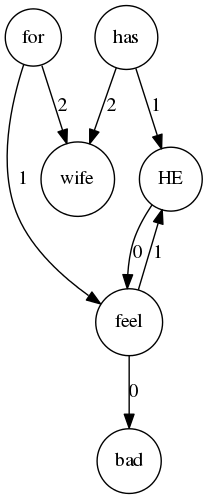
\includegraphics[scale=0.5]{figures/ifeelbad}
	\caption{\texttt{4lang} definition of sentence \textit{"I feel bad for my wife!"}.}
	\label{fig:ifeelbad}
\end{figure}

\begin{figure}
	\centering
	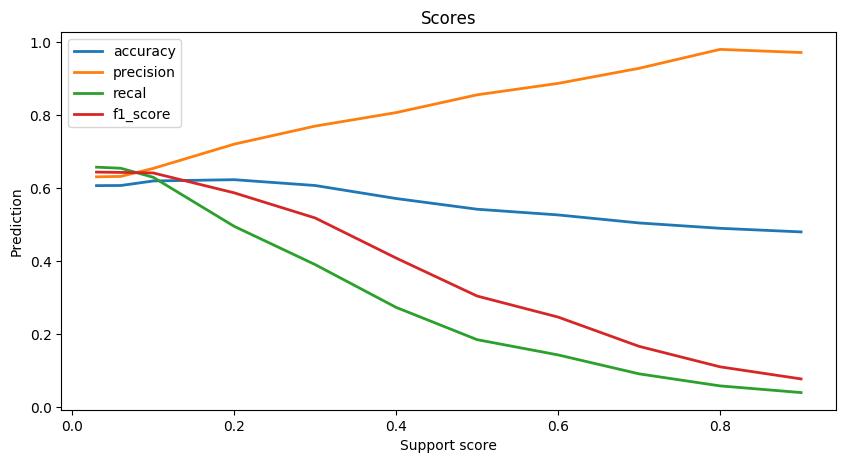
\includegraphics[scale=0.5]{figures/nlidefault}
	\caption{Baseline for the NLI task with the \texttt{default} method}
	\label{fig:nlidefault}
\end{figure}

\begin{figure}
	\centering
	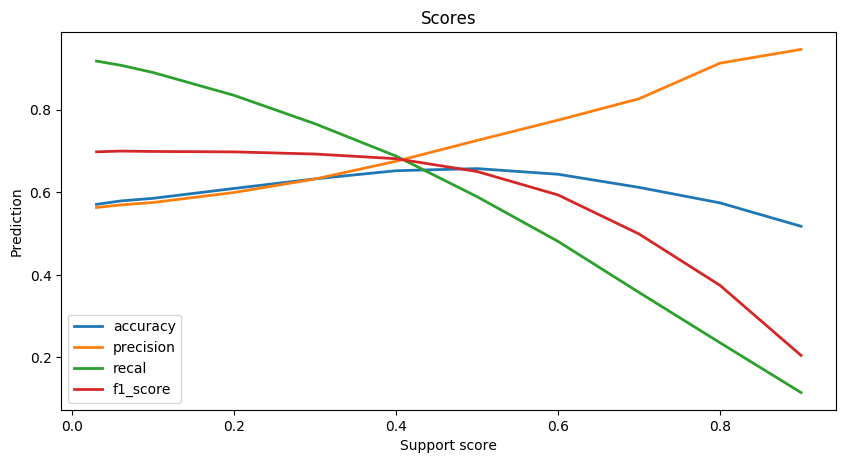
\includegraphics[scale=0.5]{figures/nliexpanded}
	\caption{Baseline for the NLI task with the \texttt{expanded} method}
	\label{fig:nliexpanded}
\end{figure}

\begin{figure}
	\centering
	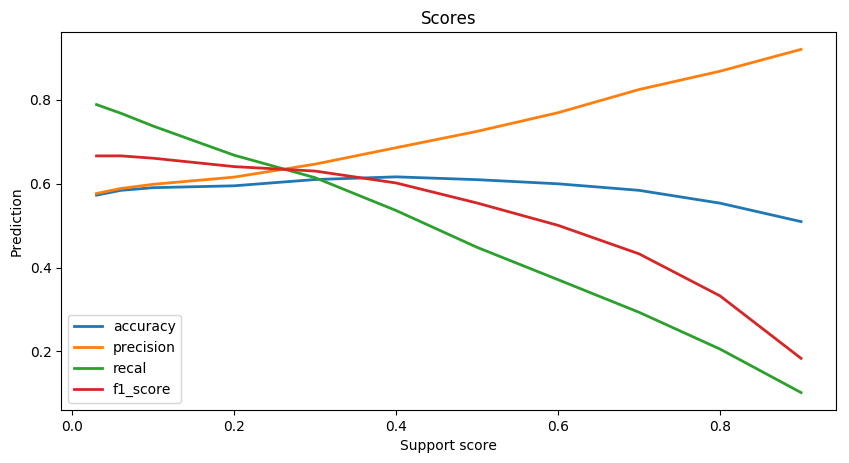
\includegraphics[scale=0.5]{figures/nliabstract}
	\caption{Baseline for the NLI task with the \texttt{substitution} method}
	\label{fig:nliabstract}
\end{figure}

\section{Substitution method}
I also had some experiments with defining new additional rules added to the \texttt{4lang} parser, that could potentially be giving us simpler definitions than the \texttt{expansion} method. It can decide if a substitution of a node in the original graph with a node from the definition graph is possible or note, meaning that a node can \textit{"fill"} the place of another node's semantic meaning. Let us look back the sentence \textit{"My poor wife"} and the expanded graph shown in Figure \ref{fig:mypoorexpanded}. In this example if we look at the edge \texttt{wife $\xrightarrow0$ woman} we can make an assumptions, that native speakers can easily make using simple inference rules \cite{Kovacs:2018} (if we state that someone is a \texttt{wife}, it also means that she is a \texttt{woman}, same can be said for \texttt{husband} and \texttt{male}). In our example, within the boundaries of the sentence we can use the concept \texttt{woman} instead of the concept \texttt{wife}. Using this simple rule we can reduce our graph to a simpler definition shown in Figure \ref{fig:mypoorabs}.

\begin{figure*}[h]
	\centering
	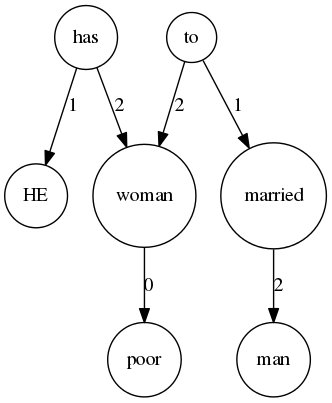
\includegraphics[scale=0.4]{figures/mypoorabs}
	\caption{Example of the \texttt{substitution} method}
	\label{fig:mypoorabs}
\end{figure*}
Let's say we have a node in our graph, and it's definition graph is also present, then I defined simple inference rules as follows:
\begin{itemize}
	\item If \texttt{X $\xrightarrow0$ Y} is present, then we can use \texttt{Y} instead of the \texttt{X} node.
	\item \texttt{Y $\xrightarrow0$ X} is present, then we can use \texttt{Y} instead of \texttt{X} node again.
	\item If we have \texttt{Y $\xleftarrow1$ Z $\xrightarrow2$ X}  both in the definition and the sentence graph, than we can connect every edge from \texttt{X} and \texttt{Y} from the definition graph to the sentence graph.
\end{itemize}
For the third rule, let's have the graph shown in Figure \ref{fig:thirdrule}, and say we have the definition of the concept \texttt{increase} in the graph in Figure \ref{fig:thirdrule2}, then by the rule number 3 we can add  additional edges to the price concept shown in Figure \ref{fig:thirdrule3}. Using these rules I also run my method for the dataset achieving results shown in Figure \ref{fig:nliabstract}. The result shows that the method cannot achieve the accuracy of the expand model for the dataset. But I believe that using the already defined simple inference rules, and adding some new ones as well could potentially define a model, where the captured meaning can exceed our results.


\begin{figure}
	\centering
	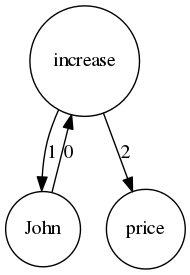
\includegraphics[scale=0.5]{figures/thirdrule1}
	\caption{\texttt{4lang} graph of \textit{"Jonh increased the price"}}
	\label{fig:thirdrule}
\end{figure}

\begin{figure}
	\centering
	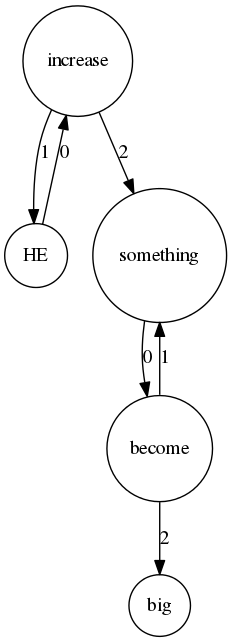
\includegraphics[scale=0.5]{figures/thirdrule2}
	\caption{\texttt{4lang} graph of the definition of \textit{"increase"}}
	\label{fig:thirdrule2}
\end{figure}

\begin{figure}
	\centering
	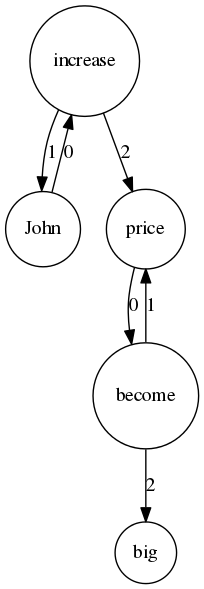
\includegraphics[scale=0.5]{figures/thirdrule3}
	\caption{Substituted graph}
	\label{fig:thirdrule3}
\end{figure}

Based on early findings I discovered using the \texttt{substitution} rules doesn't gives us better results, so in the MC task only \textit{expanded} \texttt{4lang} graphs (see
Section~\ref{sec:4lang}) was used for measuring support. 

\section{Problems}
I also found the dataset problematic for our methods, this gave me the intuition to move to the MC challenge. Few examples from the dataset, where gold label didn't imply inference, but we believe it should a form of entailment:

\textbf{premise}: \textit{European Tour, takes place at Santo da Serra Golf Club.}

\textbf{hyp}: \textit{The European tour can be found at the Santo da Serra Golf Club.}
\newline

\textbf{premise}: \textit{Thorn and the Kal will help prepare the spikes.}

\textbf{hyp}: \textit{Thor and the Kal will help the others prepare the spikes. }
\newline

\textbf{premise}:  \textit{"Heard tell as you boys don't think th' war's clear over yet,"Fenner observed.}

\textbf{hyp}: \textit{Fenner heard in the bar that these boys don't think the war is over.}
\newline

\textbf{premise}: \textit{To many Madeirans who believe the Lady of Monte has carried them through troubled times, the pilgrimage is an obligation.}

\textbf{hyp}: \textit{Because the Lady of Monte is believed to have carried them through troubled times, Madeirans believe the pilgrimage is an obligation.}
\newline
For these sentences my method yielded high \texttt{support score}, but the prediction was wrong.
Likewise some examples were found where my model didn't find any connection, nevertheless the label was entailment:

\textbf{premise}: \textit{(Emphasis added.)}

\textbf{hyp}: \textit{The emphasis was added by the editor.}
\newline

\textbf{premise}: \textit{From Beforethewars."}

\textbf{hyp}: \textit{From before the wars.}
\newline

\textbf{premise}: \textit{Ten years, sir.}

\textbf{hyp}: \textit{About a decade, sir.}
\newline

We want to move towards a goal, where our model can handle simple, trivial situations, that humans find themselves in everyday. Nevertheless I believe that these cases would not be a good base for me to rely on, because my opinion is that the defined models shouldn't be improved on cases, where even humans could argue on the right solution.

In the next chapter I will give an introduction to the MC task defining my baseline. After an introduction to the field of deep learning is discussed, followed by it's integration to a state-of-the art system, achieving a 0.5 percent improvement.